% Analyzujte nové síťové architektury jako Recursive InterNetwork Architecture (RINA) a Named Data Networking.
% Popište současný stav nasazení těchto architektur v reálném provozu i v prostředí OMNeT++. Popište jejich výhody/nevýhody.
% Implementujte modul Relaying and Multiplexing Task z RINA v prostředí OMNeT++ podle požadavků vedoucího.
% Vytvořte sadu příkladů pro demonstraci Vaší implementace. Zhodnoťte Vaše výsledky.


\chapter{Introduction}
    (\textasciitilde2 ns)

        % Network simulation is an ideal approach for examining new network architectures since it provides a quick and efficient way of setting up test scenarios and observing all aspects of their behavior. An example of a network simulator, OMNeT++, will be used for


    \section{Goals}
        The theoretical part of this thesis aims to describe and evaluate alternatives to the currently prevalent network architectures. Since the Internet is by far the largest and most important example of an internetwork, its underlying architecture shall be used as a base for comparison. This is only fitting since nearly all of the recent network architecture research is directed towards improving the building blocks of the Internet. Description of each architecture will include information about the current active implementations, both in real settings and in OMNeT++ simulation.

        The technical report describes design and implementation of a significant part of one of the presented architectures, RINA. The OMNeT++ discrete simulation framework was chosen as a target platform.

    \section{Thesis Structure}

        Part Two describes the shortcomings and weak parts of current Internet technology which create the need for alternative architecture research. This will be used further as a starting point for evaluating contributions of architectures.

        Part Three presents an outline of current projects in field of network architecture. A representative subset of network architectures will be described and evaluated.

        Part Four takes a closer look at Recursive InterNetwork Architecture, an IPC-based network architecture. It contains description of the architecture and its advantages.

        Part Five describes implementation of RINA's Relaying and Multiplexing Task in OMNeT++.

        Part Six presents evaluation of the implementation in form of sample test scenarios and their outputs.

\chapter{Problems of the current Internet}
    (\textasciitilde5 ns)

    The Internet could be, with no doubt, considered one of the most important technological achievements of the 20th century. It has brought a previously unimaginable degree of interconnection and information access to the whole world and its importance keeps growing even decades after its inception. Nevertheless, the very basic core of its technology was constructed over three decades ago in the era of first small experimental networks such as ARPANET and CYCLADES, when the the demands on internetworking capabilities were nowhere compared to now.

    During the Internet's growth, whenever there has been a problem that required a solution, it's been usually dealt with in a non-intrusive evolutionary fashion by applying a new principle on top of the underlying technology. In another words, problems have been mostly solved by adding a new protocol to the TCP/IP protocol stack. This way of improving the Internet's base technology is only logical since each paradigm shift in foundations of the Internet can require a long and expensive transfer of existing network configurations to the new technology. The most notable example of this is the internet layer protocol IPv6 requiring explicit firmware support from active network components. The problem of IPv4 space exhaustion has been known of since the beginning of 1990s, the first formal IPv6 specification arose in 1996 (RFC 2460) and the first IPv6 routers emerged in 2004 -- and yet, as of 2015, two years after the top-level IPv4 pool exhaustion, IPv6 still represents only a miniscule fraction of the total traffic on the Internet. For example, Google IPv6 adoption statistics indicate around 6\% coverage amongst the users of its services.

    As such, some of the Internet's widely recognized problems are inherent because of the base design and it's usually difficult, if not impossible, to solve them in a non-intrusive and backward-compatible way. The following sections illustrate such problems.

    \section{Router Table Size Growth}
        Default-free zone (DFZ) is the collection of all Internet autonomous systems (AS) that do not require a default route to route a packet to any destination. Since they comprise the root of the Internet's routing infrastructure, their database must be complete.

        With the increasing number of hosts connected to the Internet, the DFZ routing table sizes grow as well.

        \begin{figure}[H]
            \begin{center}
                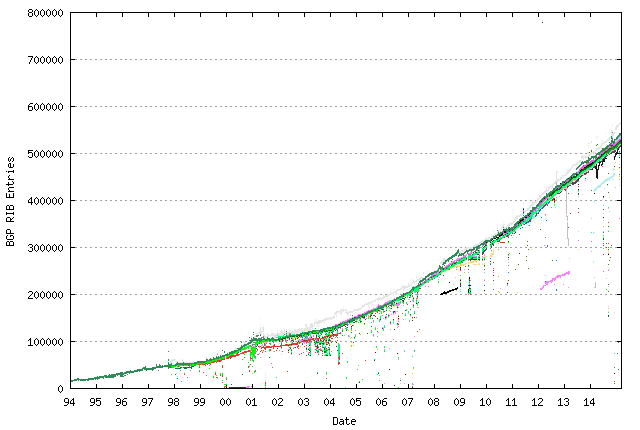
\includegraphics[width=0.6\textwidth]{fig/bgp-active.png}
              \caption{Global Internet routing table size growth}
              \label{bgp-growth}
            \end{center}
        \end{figure}


        While the exponential growth observed during the 1990s was later mitigated by mass deployment of CIDR and route aggregation, the number of items is still increasing superlinearly and the high-end router hardware needs to keep up, especially with increasing use of BGP-based multihoming and IPv6. This can sometimes lead to scalability problems, as in August of 2014 where reaching the 512k entry limit of multiple routers caused globally observable outages.

        As of year 2015, the Internet routing table is consisted of over 560k entries, which requires over 0.5 GB of memory on each router. It's been commonly believed that Moore's law will ensure that the technology of high-end routers will keep scaling along with the increased demands, but recent research proves otherwise.

    \section{Node naming}

        TODO: explain Saltzer's proposal and why it isn't used

        TCP/IP doesn't follow this proposal: the logical layer for node naming is completely missing. While the architecture does describe two distinct layers with their own address scopes (the Link Layer with physical addresses and the Internet layer with IP addresses), both types of addressing name the same thing, which is a host interface. Thus, both serve for addressing Point-of-Attachment and there's nothing to name the node itself. The need for node name->PoA resolution was eventually recognized in ARPANET and this was solved with creating a globally available file HOSTS.TXT containing mappings of alphabetic host names to IP addresses. Later on, this method was obsoleted by the Domain Name System. However, both approaches move the matter of node naming into the application layer, making applications work with location-dependent interface PoA addresses.

        The fact that the Internet effectively forwards PDUs on interface addresses and not node addresses has a great impact on difficulty of mobility and multihoming (both described in other sections). Borrowing a comparison from John Day's Patterns in Network Architecture, the lack of implicit logical addressing in the Internet ``feels like accessing memory with DOS instead of Unix''.

    \section{Lack of Multihoming}

        Since IP addresses serve as point-of-attachment addresses (i.e. one per each computing system interface) and routing is done exclusively on IP's layer, there isn't any implicit mechanism for distinguishing whether multiple IP addresses belong to a single node. The insufficient base for multihoming support is also one of the oldest recognized problems of the Internet: it has become apparent back in 1972, when Tinker Air Force Base joined ARPANET and voiced a request for redundant connections to a single node to ensure reliability. In spite of this, a switch to a new protocol suite that happened 11 years later (on the ``flag day'') didn't bring any solution to this problem.

        Since then, some attemps were made to implement multihoming on top of the current architecture.

        \subsection{SCTP}
        Message-oriented transport protocol SCTP provides a partial support. Two SCTP hosts are able to provide each other with lists of alternate IP addresses that can be used as fallback points of attachment of the same application in case of failure of the primary address. During such session, each SCTP host needs to continually check other host's endpoints by heartbeat packets to make sure they are accessible via other sessions. However, thus far, multiple reasons have been preventing SCTP from becoming a widely known and used solution; the biggest disadvantage lies in the fact that due to TCP/IP not having a distinct session layer on top of its transport layer (such as in ISO/OSI stack), the transport protocol must be explicitly specified by the application using sockets API. Therefore, SCTP adoption would require a rewrite of network-aware applications themselves. Other SCTP adoption issues include unsatisfactory operating system support (Microsoft Windows systems require a third-party kernel driver) and weak awareness of its existence outside the networking community.

        \subsection{BGP Multihoming}
        Another implementation of multihoming capabilities can be seen in Border Gateway Protocol, which provides means for load-balancing and fallback over multiple links on T1 networks. To make use of such multihoming over the Internet, a public IP address range and an Autonomous System number are required. BGP Multihoming is one of the most significant causes contributing to the growth of Internet routing table.

        \subsection{Multipath TCP}
        The most recent TCP/IP multihoming initiative is the TCP extension Multipath TCP (MPTCP) which is currently in its experimental phase, although a large scale commercial deployment has been already made by Apple for its Siri network application in mobile operating system iOS 7.

    \section{Lack of Mobility}

        Since a host location is determined by its IP address and IP addressing is location-dependent, mobility using re-locatable addresses is essentialy non-existent.

        TODO: MobileIP

    \section{Lack of security mechanisms}
        The specifications of the fundamental protocols of TCP/IP stack -- IP, TCP and DHCP -- were originally finished at the beginning of 1980s. Computer internetworking in pre-Internet era was still a matter of closed research exercised in small scientific communities, so most of the design effort was given to making things work and network security wasn't the main aim. However, the Internet has since then turned into a massive world-wide internetwork connecting people of different types and agendas. Naturally, once the Internet began to be used for transferring sensitive data (especially by companies), cyber crime started to emerge as well and some attention was turned to security aspects of Internet protocol (or lack thereof).

        Over the decades, a large amount of security flaws has been discovered and continually exploited. Some examples of these are Denial-of-service attacks (ICMP flood, SYN flood, CAM flood), Man-in-the-Middle attacks, IP address spoofing, DHCP spoofing, ARP spoofing and ARP cache poisoning. The requirement of every secure network is to carefully mitigate all of them.

\chapter{Overview of Alternative Architectures}
    (\textasciitilde12 ns)

    This chapter gives an overview of paths that were pursued in the field of network architecture research.

    Considering the limited scope of this thesis, only a representative subset of currently researched network architectures (namely, the architectures emerged under the Future Internet Architecture project) will be described more thoroughly and evaluated.

    \section{Design Approaches}

        Over the past several years, the networking research community has exhibited many attempts of moving the field forward. The undertaken research directions are often classified into one of two groups:

        \begin{itemize}
            \item evolutionary design: backward-compatible solutions that are incrementally deployable on top of the current Internet (e.g. SDN, LISP, DiffServ, IntServ), or
            \item clean slate design: designing completely new standalone architectures that aren't constrained by Internet technology's limitations (e.g. NDN, RINA)
        \end{itemize}

        Considering the scope of this thesis, the focus will be given exclusively to ``clean-slate design'' architectures.

    \section{Research Initiatives}

        TODO: a brief overview + focus on FIA

        \subsection{NewArch Project}
        \subsection{FIRE}
        \subsection{FIBRE}
        \subsection{Future Internet Architecture}
            In 2010, National Science Foundation funded five projects as a part of this program: Named Data Networking, MobilityFirst, NEBULA, eXpressive Network Architecture and ChoiceNet.


    \section{Named Data Networking}
        (\textasciitilde8 ns)
        \subsection{Premise}
            As described in section 2.1, the current Internet has its roots in telecommunication technology as this was the only area from which any inspiration could be taken. Because of this, technology of the Internet has been built on the paradigm of host-to-host communication. This can be visually presented on an ``hourglass model'', which indicates that while there's a wide array of technologies in use in the lower and higher layers, the hourglass's thin waist of end-to-end communication exercised by the IP protocol is the key static part binding different networks together.

            \begin{figure}[H]
                \begin{center}
                    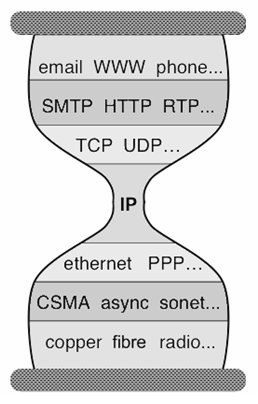
\includegraphics[width=0.2\textwidth]{fig/ndn_hourglass1.jpg}
                  \caption{Internet's ``thin waist''}
                  \label{ndn-hourglass1}
                \end{center}
            \end{figure}


            Building the Internet as a communication network was an obvious choice, especially since most of communication of the early ARPANET consisted of connecting terminals to mainframes and executing remote procedures on them.

            However, while the basic paradigm of host-to-host communication hasn't changed, the way we use the Internet has gone in an entirely different direction: the Internet has become mostly a content distribution network. Since the mechanism of communication over the Internet is based on creating and maintaining end-to-end connections, this creates an enormous amount of data redundancy.

            Named Data Networking proposes a solution for the problem: instead of working with the source/destination node identifiers, the ``thin waist'' of the Internet should work with names of data chunks.

            \begin{figure}[H]
                \begin{center}
                    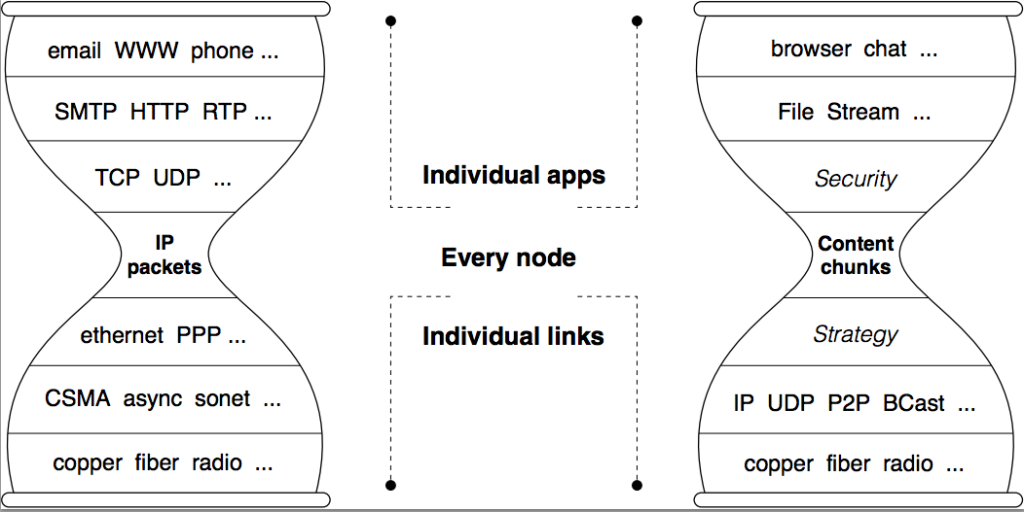
\includegraphics[width=0.6\textwidth]{fig/ndn_hourglass2.png}
                  \caption{NDN's ``thin waist''}
                  \label{ndn-hourglass2}
                \end{center}
            \end{figure}

        \subsection{Concepts}
            \subsubsection{The Building Blocks}
                The NDN architecture specifies:
                    \begin{itemize}
                        \item two types of packets: an interest packet (containing the name of desired data) and a data packet (containing the requested data)
                        \begin{figure}[H]
                            \begin{center}
                                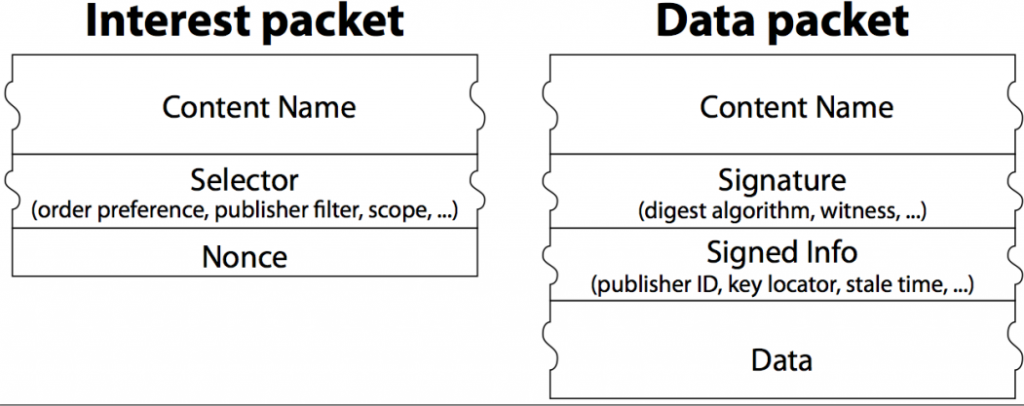
\includegraphics[width=0.6\textwidth]{fig/ndn_packets1.png}
                              \caption{NDN packet types}
                              \label{ndn-packets}
                            \end{center}
                        \end{figure}
                        \item two types of hosts: a consumer (data requester) and a producer (data provider)
                        \item a router maintaining three fundamental data structures:
                        \begin{itemize}
                            \item Forwarding Information Base (forwarding table)
                            \item Pending Interest Table (maintaining currently active requests)
                            \item Content Store (data cache)
                        \end{itemize}
                        \begin{figure}[H]
                            \begin{center}
                                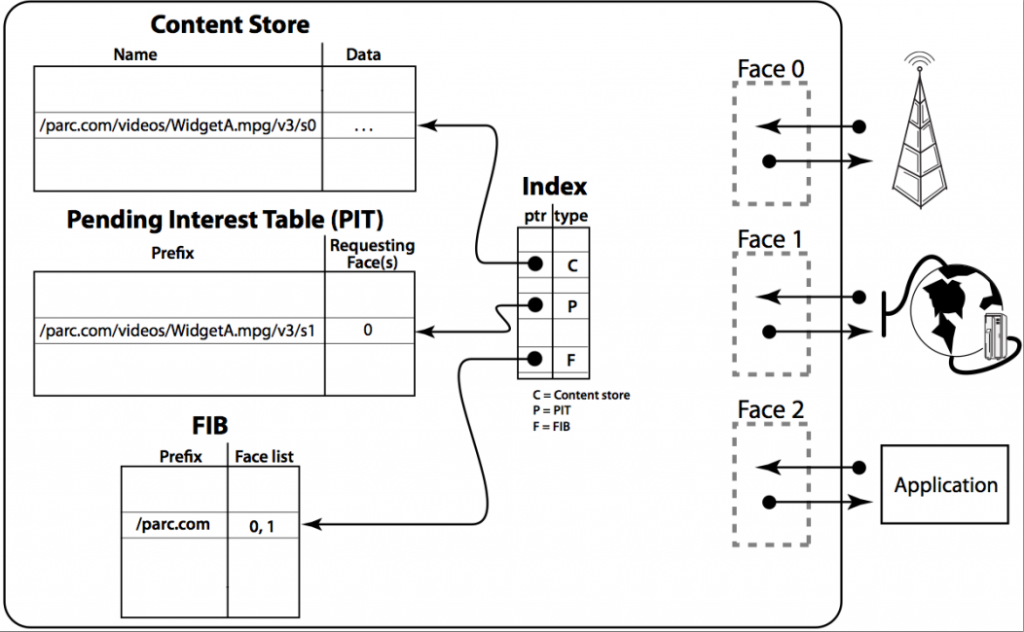
\includegraphics[width=0.6\textwidth]{fig/ndn_router1.png}
                              \caption{NDN router}
                              \label{ndn-router1}
                            \end{center}
                        \end{figure}

                    \end{itemize}

                \subsubsection{The Communication Model}

                Communication in NDN is driven by the data receiver, i.e. consumer.

                \begin{enumerate}
                    \item The consumer sends out an ``interest packet'' containing the name of the desired data.
                    \item When a router receives the interest packet, it first consults its Content Store for requested data.
                        \begin{itemize}
                            \item If the data requested by the interest packet are present, they are returned in the direction of the requesting interface.
                            \item Otherwise, it'll look up the Pending Interest Table.
                            \begin{itemize}
                                \item If there's an entry present for the named data request, the entry is updated by adding the originating interface into the list of requesting interfaces, thus aggregating the new request together with an existing one.
                                \item Otherwise, a new entry is inserted, a FIB lookup is made and the interest packet is forwarded to interface(s) returned by the FIB.
                            \end{itemize}
                        \end{itemize}
                    \item A data packet is returned to the router by either the producer or another router with cached data. The router finds a matching PIT entry and forwards the data to all interfaces listed in the PIT entry. The PIT entry is then removed and data are cached into the Content Store.
                \end{enumerate}

        \subsection{Implications}
            \subsubsection{Data Caching}
                The most significant feature of NDN is its native support for caching all sorts of data inside the network itself. While this should be beneficial mostly for static data such as web pages and images, dynamic content could take advantage of this as welll in case of multicasting or packet retransmission on packet loss.

            \subsubsection{Routing and Forwarding}
                NDN routes and forwards packets on names, which eliminates four problems caused by address forwarding in the IP architecture: address space exhaustion, NAT traversal, mobility, and address management.
                \begin{itemize}
                    \item There is no address exhaustion problem since the namespace is unbounded.
                    \item There is no NAT traversal problem since a host does not need to expose its address in order to offer content.
                    \item Mobility, which requires changing addresses in IP, no longer breaks communication since data names remain the same.
                    \item Finally, address assignment and management is no longer required in local networks, which is especially empowering for embedded sensor networks.
                \end{itemize}

                Since the forwarding mechanism otherwise bears a strong resemblance to the forwarding mechanism in IP networks, lot of the existing research on IP routing could be applied to NDN as well: protocols like BGP, IS-IS or OSPF can be, for the most part, reused with minor modifications (e.g. routers would announce name prefixes instead of IP prefixes).

            \subsubsection{Security}
                While TCP/IP with its end-to-end communication paradigm relies on setting up a secure channel between two hosts and transmitting data through it, NDN requires each data chunk to be signed together with its name. Thus, since security is built into the data itself, there's no need for a direct host-to-host secure channel to be created.

        \subsection{Current State of Implementation}


    % \section{NFN}
    %     TODO: probably purge this one

    %     NFN's founders present it as ``a companion project to Named Data Networking''. While CCN (and, in turn, NDN) is based on the idea of resolving names to content, NFN decides to take an even more general approach: resolving names to computations.

    \section{eXpressive Network Architecture}

        \subsection{Premise}
            As presented in the previous sections, some of the future architecture research is centered around the idea of replacing Internet's narrow waist of end-to-end communication with a different principal (e.g. NDN and its named content). XNA takes this approach one step further and builds on one basic premise: the narrow waist should provide support for multiple principals and the ability to evolve its functionality to accomodate new principals over time.


    \section{NEBULA}
        \subsection{Premise}
        \subsection{Current State of Implementation}

    \section{MobilityFirst}
        \subsection{Premise}
            % The current Internet is designed for interconnecting fixed endpoints and fails to address the trend of dramatically increasing demands of mobile devices and services. MobilityFirst, as its name would suggest, aims to abandon this approach and make

        \subsection{Current State of Implementation}

    \section{ChoiceNet}
        \subsection{Premise}
        \subsection{Current State of Implementation}

    \section{Recursive InterNetwork Architecture}


    \section{Comparison \& Evaluation}
        some nice tables + a paragraph or two


\chapter{Recursive InterNetwork Architecture}
    (\textasciitilde8 ns)
    In 2008, computer scientist John D. Day has published a book that marked the culmination of his long-time goal of rediscovering the way we think about computer networks. The book is called Patterns in Network Architecture and in it, Day proposes a clean-slate approach to computer architecture that aims to get rid of most of TCP/IP's drawbacks.

    The book can be roughly divided into two parts: in the first part, Day attempts to decompose mechanisms used in TCP/IP to their basic parts and put them into historical and socio-economical context. The second part takes into account all of the fundamentals discovered in the first part and uses them as foundations to build an entirely new concept of network architecture from scratch: the recursive IPC model (originally Network IPC Architecture, NIPCA).

    Recursive InterNetwork Architecture (RINA) is a currently researched network architecture based on fundamental principles described by Day.

    This chapter describes the motivation behind RINA and its basic principles. Special attention will be given to its Relaying and Multiplexing Task as the technical report part of this thesis deals with its implementation.

    \section{Premise}
        The very basic principle of RINA could be summed up in one sentence: Networking is a recursively scalable set of distributed applications specialized to do inter-process communication.

    \section{Building blocks}
        The basic principles of RINA are documented in form of a mental exercise. In the beginning of the second part of his book, Day begins to construct a new networking paradigm by starting at the simplest possible scenario of communication between two applications (IPC inside a system) and then gradually increasing scenario complexity to the point where it can be used as a complete internetworking paradigm.

        \vspace{300pt}
        Simple IPC communication requires

        Then, Day moves to the next scenario: two applications in two distinct systems commmunicating with each other.

        This brings the need for multiple new features:

        \begin{itemize}
        \item Name space management is no longer under the control of a single system, hence there's a need for a protocol to carry application names and access control information, IAP.
        \item Since there's a possibility of data getting lost or corrupted on transit, there's a need for a transfer protocol to handle it: EFCP.
        \end{itemize}

        Since the days of single-application hosts are long gone, the next scenario specifies a case of simultaneous communication between two systems.
        \vspace{300pt}
        \begin{itemize}
        \item EFCP instances now require means to distinguish one flow from another, so source and destination ports are included in the IAP protocol header.
        \item Since EFCP instances need to concurrently use a single resource ((N-1)-flow or a physical layer protocol), a multiplexing application is defined.
        \item Applications can run in multiple instances, an Application Instance name is included.
        \end{itemize}

        The next step is making a host to be able to communicate with more then one system. The simplest approach is a full mesh where each host in a network is directly connected to every other host in a network
        \vspace{300pt}
        \begin{itemize}
        \item Since different media may require different management, each of them will be put in a separate (N)-DIF and there will be another (N+1)-DIF on top of them to manage (N-1)-flows and provide a media-independent facility to the applications.
        \item We need to locate which applications are reachable via which interfaces -- hence, a directory maintaing mappings of application names to IPC addresses is needed.
        \end{itemize}

        While communication with multiple host is now feasible, the brute-force approach of N:N connections is expensive and doesn't scale. Hence, we should dedicate certain systems to relay PDUs between destinations.
        \vspace{300pt}
        \begin{itemize}
        \item Since different media may require different management, each of them will be put in a separate (N)-DIF and there will be another (N+1)-DIF on top of them to manage (N-1)-flows and provide a media-independent facility to the applications.
        \item We need to locate which applications are reachable via which interfaces -- hence, a directory maintaing mappings of application names to IPC addresses is needed.
        \end{itemize}

        At this point, all building blocks are in place to construct networks based on distributed IPC.

    \section{Design Principles}
        Day's architecture is based on a set of principles justified in the first part of his book.

        \subsection{Connection-less vs. Connection-oriented}
            function of IPC, not part of application API, bla bla

        \subsection{Delta-T}



        \subsection{Separation of mechanism and policy}

            Day's favorite example of such approach in practice is the Telnet protocol: instead of creating two distinct variations of Telnet for x and y, Telnet supports both and the decision of whether or not to use them is up to the policy. Thus, Telnet is an example of distinct mechanisms being encompassed as policies inside a common general mechanism.

            Thanks to its strict separaton of mechanisms and policies, one of the most important selling points of RINA is its flexibility -- RINA provides a framework for implementing diverse set of paradigms for flow control and network management  ...

    \section{Forwarding and Routing}
        Each IPC process has to solve the forwarding problem: given a set of EFCP PDUs and a number of (N-1)-flows leading to various destinations, to which flow should each PDU be forwarded? In RINA, the decision is handled by the Relaying and Multiplexing task and its PDUForwardingPolicy. The PDUForwarding policy may consist of looking up the PDU's destination in its forwarding table (resembling the forwarding mechanism in traditional TCP/IP routers), but it's not a requirement; other experimental forwarding paradigms (such as forwarding based on topological addressing) may not require a forwarding table at all and .

        When in need of deciding for an output (N-1)-port for a PDU, the PDUForwardingPolicy is given the PDU's PCI and in turn returns a set of (N-1)-ports to which the PDU has to be sent. This provides enough granularity to implement multiple communication schemes apart from unicast (such as multicast or load-balancing), because the decision is left to the PDUForwardingPolicy. E.g. a simple forwarding policy would return a single (N-1)-port based on PDU's destination address and QoS-id, whereas in case of a load-spreading policy and multiple (N-1)-ports leading to the same destination, the policy could split traffic by PDUs' flow-ids and always return a single (N-1)-port from the set.

        Generating information necessary for PDUForwardingPolicy is one of the tasks of IPC process's Resource Allocator, namely its subcomponent called PDU Forwarding Table Generator. For this purpose, Resource Allocator generally uses pieces of information provided by other sources, most notably the Routing Policy.

        The Routing Policy exchanges information with other IPC Processes in the DIF in order to generate a next-hop table for each PDU (usually based on the destination address and the id of the QoS class the PDU belongs to). The next-hop table is then converted into a PDU Forwarding Table with input from the Resource Allocator's PDU Forwarding Table Generator, by selecting an N-1 flow for each ``next-hop''. The Routing Policy may resemble distance vector and link-state routing protocols used in today's Internet, but the current research is also aimed at other paradigms such as topological/hierarchical routing, greedy routing or MANET-like routing.

    \section{Relaying and Multiplexing Task}

        \subsection{Formal description}

            Relaying and Multiplexing Task (RMT) has, as its name suggests, two main reponsibilities: relaying and multiplexing of PDUs. The goal of multiplexing is to simply pass PDUs from EFCP instances and RIB to the appropriate (N-1)-flows (and reverse of that). Relaying handles incoming PDUs from (N-1)-ports that aren't directed to its IPC process and forwards them to other (N-1)-ports using information provided by its forwarding policy.

            \vspace{300pt}

            RMT instances in hosts and bottom layers of routers usually perform only the multiplexing task, while RMTs in top layers of interior/border routers do both multiplexing and relaying. In addition to that, RMTs in top layers of border routers perform flow aggregation.

            \vspace{300pt}

            Each (N-1)-port handled by RMT has its own set of input and output buffers. The number of buffers, their monitoring, their scheduling discipline and classification of traffic into distinct buffers are all matter of policies.

            RMT is a straightforward high-speed component. As such, most of its management (state configuration, forwarding policy input, buffer allocation, data rate regulation) is handled by the Resource Allocator which makes the decisions based on observed IPC process performance.


        \subsection{Policies}
            Even though Relaying and Multiplexing Task serves as a low-overhead component similar to the traditional view of router data plane, several policies are defined for modifying its behavior.

            \begin{itemize}
                \item RMT scheduling policy. A scheduling algorithm (also commonly known as ``network scheduler algorithm'' or ``queuing discipline'') that determines the order input and output buffers are serviced. This policy should be invoked each time a PDU needs to be taken from a queue for processing and works for both input and output directions. Examples of possible algorithms could be FIFO, LIFO or Fair Queuing.
                \item RMT monitoring policy. A queue monitoring algorithm that is invoked each time a PDU enters or leaves a queue. This policy should compute variables to be used in decision process of other policies. Examples of such variables could be average queue length or queue idle time, which are often used by congestion prevention mechanisms.
                \item RMT max queue policy. An algorithm that is invoked each time the number of PDUs waiting in a queue exceeds the queue's threshold. This policy is mostly used for implementing congestion control mechanisms (e.g. by dropping or marking the last PDU in a queue).
            \end{itemize}


    \section{Implications}
        In many aspects, RINA is fundamentally different from the other research initiatives. While other alternative architectures, likes of which were described in the previous chapter, were concieved under a research grant and focused just on one or few distinct problems described in Chapter 2, RINA started as a lone scientist's free-time things and in an almost incidental manner it provides a solution for the biggest problems with the current Internet.

    \section{Current State of Implementation}
    \section{Evaluation}

        The main drawback with adoption of RINA isn't implementation (incremental deploymend with RINA Sockets API is in progress), but in the complete paradigm shift which throws away most of the progress done in field of TCP/IP research.


\chapter{Implementation of Relaying and Multiplexing Task}
    (\textasciitilde10 ns)
    \section{OMNeT++}
        OMNeT++ is an open-source discrete simulation framework used primarily in the field of network simulation. In this context, the term ``network'' refers to the more general meaning of the word, which means that apart from simulating TCP/IP (especially in conjecture with the INET library) and other computer networks, it also provides means for simulating other networked systems such as on-chip networks or queuing networks. As we're implementing a clean-slate architecture from the ground up, this is an ideal approach.

        OMNeT++ provides a component architecture for models. Components (modules) are programmed in C++, then assembled into larger components and models using the high-level language NED. In theory, there are no limits for networks modelled by NED and the only constraint is given by the computing platform processing power.

    \section{RINASim}
        RINASim, developed by networking research group at Faculty of Information Technology of Brno University of technology, is an open-source OMNeT++ library developed for project PRISTINE. The purpose of the library is to provide a framework for building RINA networks and observing their behavior. In the current stage of initial development, RINASim is used primarily by other PRISTINE researchers to experiment with the architecture and efficiently evaluate their working theories.

        The library is open-sourced with MIT licence and publicly hosted by GitHub.

    \section{Process of development}
        Since RINA is still an emerging architecture, some of its parts (e.g. SDU Protection) are still being actively worked on and the current implementations aren't yet fit for production purposes. Hence, there wasn't much to rely on when implementing RMT: the specifications were brief, implementation design non-existent and the only existing implementations were providing only a small subset of RMT's functions. Because of this, most of the later phase of development was driven by PRISTINE researchers' feature requests and frequent mutual feedback regarding architectural or implementational issues.

    \section{Implementation Design}

        In RINASim, all functionality of RMT including a policy architecture is encompassed in a single compound module named ``RelayAndMux'' which is present in every IPC process. The module serves for (de)multiplexing, relaying and aggregating PDUs of data flows traversing the IPC processes.

        \subsection{Module Structure}

            \begin{figure}[H]
                \begin{center}
                    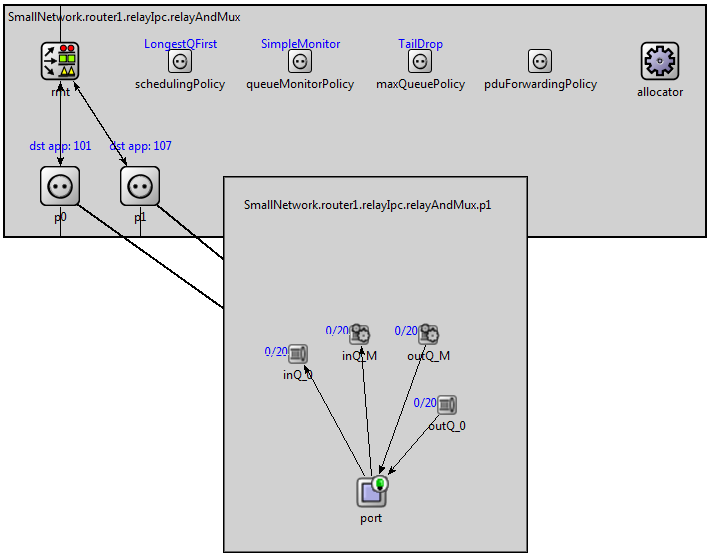
\includegraphics[width=0.8\textwidth]{fig/rmt_all.png}
                  \caption{RelayAndMux module contents}
                  \label{omnet-rmt}
                \end{center}
            \end{figure}

            RelayAndMux consists of multiple simple modules of various types, some of which are instantiated only dynamically at runtime.

            Static modules:
            \begin{itemize}
                \item RMT, the central logic of Relaying And Multiplexing task that decides what should be done with messages passing through the module.
                \item RMTModuleAllocator, a control unit providing an API for adding and deleting instances of dynamic modules (RMTQueue, RMTPort).
                \item SchedulingPolicy, a scheduling policy of an RMT instance.
                \item MonitorPolicy, a monitoring policy of an RMT instance.
                \item MaxQPolicy, a maxqueue policy of an RMT instance.
            \end{itemize}

            Dynamic modules:
            \begin{itemize}
                \item RMTPort, a representation of one endpoint of an (N-1)-flow.
                \item RMTQueue, a representation of either input or output queue. The number of RMTQueues per RMTPort is determined by Resource Allocator policies.
                \item RMTPortWrapper, a compound module encapsulating an (N-1)-port and its queues.
            \end{itemize}

            ER.png

        \subsection{Module Parameters}
            Some of the modules contain user-configurable parameters that can be used to alter their behavior. % The whole list of parameters can be found in attachment A2.
            \begin{itemize}
                \item par1
                \item par2
                \item par3
            \end{itemize}


        \subsection{Module Workflow}
            diagrams, descriptions, pie charts etc.

            - add PDU traversal in OMNeT

            \begin{figure}[H]
                \begin{center}
                  \makebox[\textwidth]{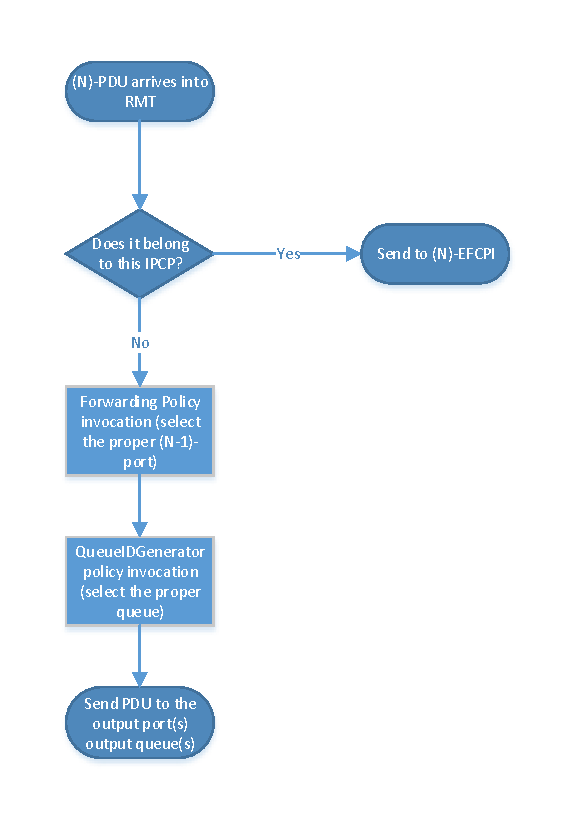
\includegraphics[width=\paperwidth/3]{fig/rmt.pdf}}
                  \caption{The core RMT FSM}
                  \label{rmt-fsm}
                \end{center}
            \end{figure}

            \begin{figure}[H]
                \begin{center}
                  \makebox[\textwidth]{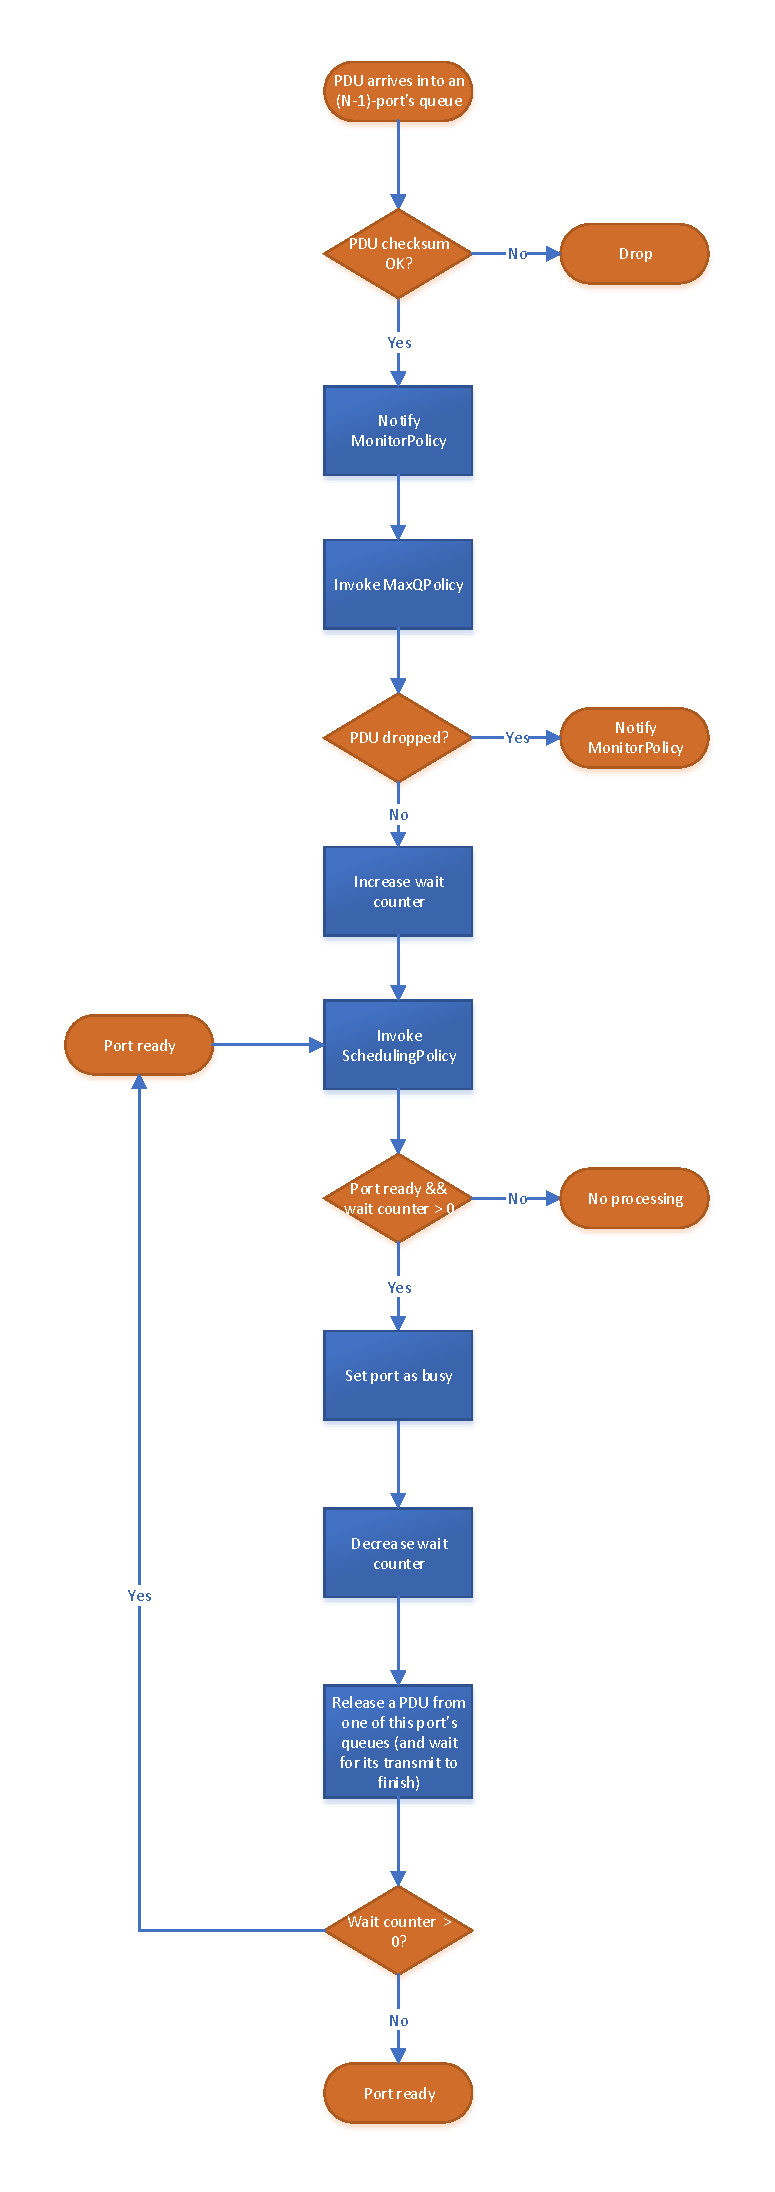
\includegraphics[scale=0.6]{fig/sched.pdf}}
                  \caption{Scheduling FSM}
                  \label{scheduling-fsm}
                \end{center}
            \end{figure}

        \subsection{Module Management}
            RMT's purpose in an IPC process is fairly straightforward: providing a stateless function for relaying PDUs to their predetermined destinations and multiplexing PDUs of multiple data flows onto a common predetermined medium. The entire management of the RMT is decoupled and exercised by some of the functions of the Resource Allocator. This includes tasks such as:

            \begin{itemize}
                \item Initial setup of RMT mode of function. When a RMT instance is located inside a bottommost IPC process that doesn't work with any further (N-1)-IPC processes, the RMT is switched to an ``onWire'' mode that functions over a simple medium instead of an IPC connection.
                \item Forwarding table management. The content of the PDU forwarding table is generated by the PDU Forwarding Table Generator module which generally exchanges routing information with other IPC processes by some sort of routing protocol.
                \item Queue allocation. PDUs traversing an (N-1)-port may be momentarily buffered in input or output queues; the number of input and output queues per (N-1)-port and assignment of traffic classes to queues (e.g. all-in-one or fair queuing) is determined by Resource Allocator policies.
                \item (N-1)-port creation \& removal. Since Resource Allocator manages (N-1)-flows with other IPC processes, it also provides (N-1)-ports (or handles) for RMT.
                \item (N-1)-port data rate control. In some scenarios, it may be required for an (N-1)-port to cease/slow down sending or providing more data because of congestion. Resource Allocator can momentarily disable or slow down data rate on distinct ports if this is required by EFCP instances.
            \end{itemize}

        \subsection{Statistics Collection}
            OMNeT++ modules provide means for declaring scalar or vector NED variables used for statistics collection. Processing of such statistical data (e.g. generating summaries and graphs) is decoupled from the act of data collection itself, so it's up to the user to pick out which data he wants to work with.

            Since the Relaying and Multiplexing Task is the shared point of data flow traversal in the IPC process, it's well-suited for monitoring data flow performance. Several statistical variables have been defined for this very purpose:

            \begin{itemize}
            \item (N-1)-port PDU traversal count. Two scalar variables for both input and output containing the number of PDUs transferred through the port in each direction.
            \item RMT queue length. A vector variable documenting number of PDUs in a queue over time.
            \item RMT queue drop count. A scalar variable providing the number of PDUs dropped by a queue.
            \end{itemize}

            Multiple examples of graphs generated from the variables can be seen in the next chapter.

    \section{}


\chapter{Testing and Evaluation}
    (\textasciitilde4 ns)

\chapter{Conclusion \& Future Development}
    (\textasciitilde1 ns)

    everyone's happy :-*

    possible extensions: RA policies for QoS monitoring
